\documentclass[root.tex]{subfiles}
\begin{document}



\section{Solution de contrôle du bras UR5 développée sous Windows}

Le contrôle du bras UR5 sous windows présente quelques défis puisque la majorité des outils de développement pour cet équipement sont développés sur la plateforme Linux.
Sachant que cette plateforme est souvent méconnue, la solution développée pour interagir avec le bras tentera de minimiser le travail requis avec Linux et fera le lien entre Matlab, URsim et un logiciel de visualisation ce nommant VRep. 
Ce dernier permet l'insertion et la visualisation de différents objets dans l'environnement du robot puisque URsim ne peut que représenter le robot lui-même.
Tout d'abord, cette section expliquera l'installation de URsim et les différentes fonctionnalités utiles à la mise en place de l'infrastructure.
Ensuite, le moyen de communication entre Matlab et URsim sera décrit.
Finalement, l'interaction avec le logiciel de visualisation VRep sera expliqué.

\subsection{URsim et son utilisation}

URsim permet l'interface avec un robot virtuel ou un robot réel connecté sur le réseau.
Cette caractéristique est importante puisqu'il serait relativement facile de faire un simulateur directement dans matlab, cependant ce dernier ne pourrait pas directement contrôler le bras UR5.
En utilisant URsim, le robot simulé agit directement comme un vrai robot, simulant les limitation de forces, de courant et les arrêts d'urgences.
Ce logiciel permet la programmation de routines de base ainsi que la définition de fonctions plus complexe permettant, entre autre, la communication UDP avec d'autre logiciels.
URsim, en soit, n'est disponible que sur Linux.
Cependant, sur le site web de l'entreprise \href{https://www.universal-robots.com/download/}{Universal Robots}, une machine virtuelle sur laquelle URsim est déjà installée est disponible.
Ceci permet de conserver l'environnement de développement Windows en exécutant URsim dans une machine virtuelle Linux.
Le logiciel avec lequel cette machine virtuelle a été utilisée pour l'environnement de développement a été VmWare.
Suite au lancement de la machine virtuelle et d'URsim, l'interface initiale d'URsim vous est présentée (Figure \ref{fig:ui_start}).

\begin{figure}
 \begin{center}
  \begin{tabular}{c}
    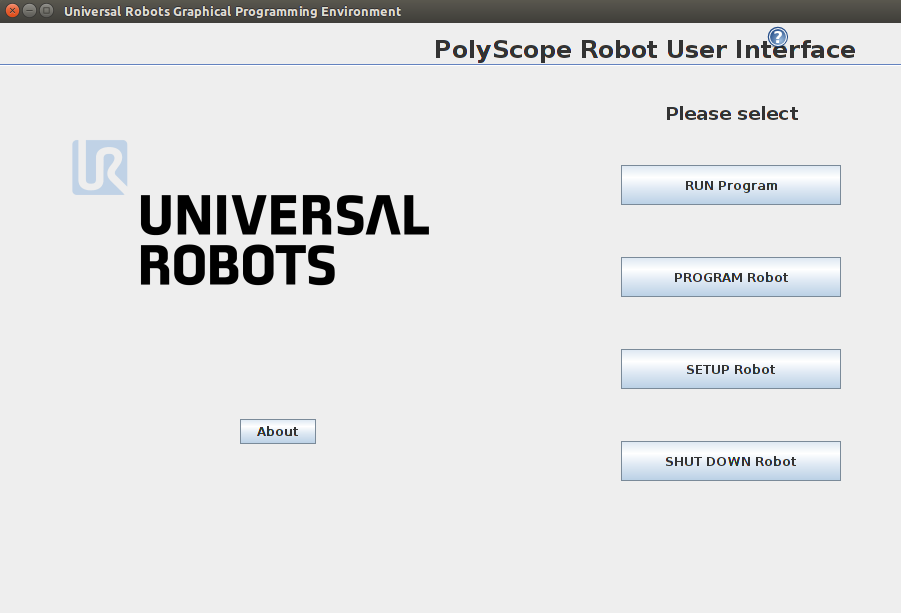
\includegraphics[trim=0cm 0cm 0cm 0cm, scale=0.4]{screenshots_tuto_ursim/interface_init.png}
  \end{tabular}
 \end{center}
\caption{Interface initiale d'URsim}
 \label{fig:ui_start}
\end{figure}

\begin{itemize}
\item Le bouton \textit{RUN Program} permet de faire fonctionner des routines contenant différentes fonctions. Ces routines sont communément appelées \textit{URscript}. Ces scripts peuvent variés en complexité allant d'une simple séquence de positions à atteindre jusqu'à un programme complexe gérant de multiples sockets de communications UDP et répondant à des appels de fonctions listées dans la librairie d'URsim.
\item Le bouton \textit{PROGRAM Robot} permet la rédaction ou la modification d'URscripts
\item Le bouton \textit{SETUP robot} permet la modification de paramètres tels que l'adresse IP d'un robot réel qu'un utilisateur voudrait contrôler via l'instance d'URsim installée sur la machine virtuelle.
\end{itemize}

Quand un utilisateur charge un URscript, il appui alors sur \textit{PROGRAM ROBOT}, puis sur \textit{Load Program} (ou sur \textit{Empty program} si il n'y a pas de programmes déjà disponibles). Une fois cette opération complétée la fenêtre présente à la Figure \ref{fig:ui_programmation}. Ceci constitue l'interface de programmation d'URscripts. Un manuel de programmation URscript est inclue dans l'appendice A, cependant, pour le fonctionnement de l'environnement de développement tel que présenté, aucune programmation URscript ne sera nécessaire.

\begin{figure}
 \begin{center}
  \begin{tabular}{c}
    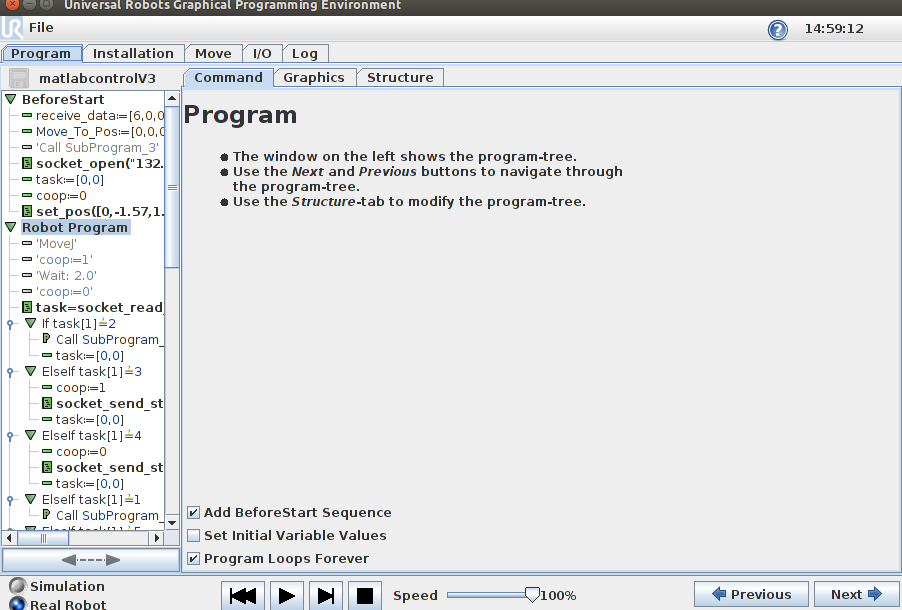
\includegraphics[trim=0cm 0cm 0cm 0cm, scale=0.45]{screenshots_tuto_ursim/interface_prog.png}
  \end{tabular}
 \end{center}
\caption{Interface de programmation d'URsim}
 \label{fig:ui_programmation}
\end{figure}



\subsection{Lien URsim-Matlab}
Comme mentionné précédemment, les URscripts peuvent gérer des sockets de communication UDP et utiliser des fonctions tirées de la librairie d'URsim. 
En premier lieu, les manipulations requises dans le logiciel URsim lancé dans la machiner virtuelle seront décrites.
Ensuite, les étapes à suivres dans l'environnement de développement Matlab sous windows seront expliquées.

\subsubsection{Manipulations dans URsim}

Un URscript a été rédigé afin de permettre à URSIM de répondre à certaines commandes envoyées sous format texte via Matlab.
Les fichiers URscripts en question sont disponibles dans le dossier \textit{programs} du dépot github \href{https://github.com/wonwon0/code_sujet_special}{suivant}.
Pour rendre ces URscripts disponibles pour URsim, il faut seulement remplacer le dossier \textit{programs} présent dans le répertoire d'instalation d'URsim par celui téléchargé depuis le répertoire github mentionné plus haut. La figure \ref{fig:programs} représente grosso modo l'endroit dans lequel il faut remplacer le dossier \textit{programs}.
\begin{figure}
 \begin{center}
  \begin{tabular}{c}
    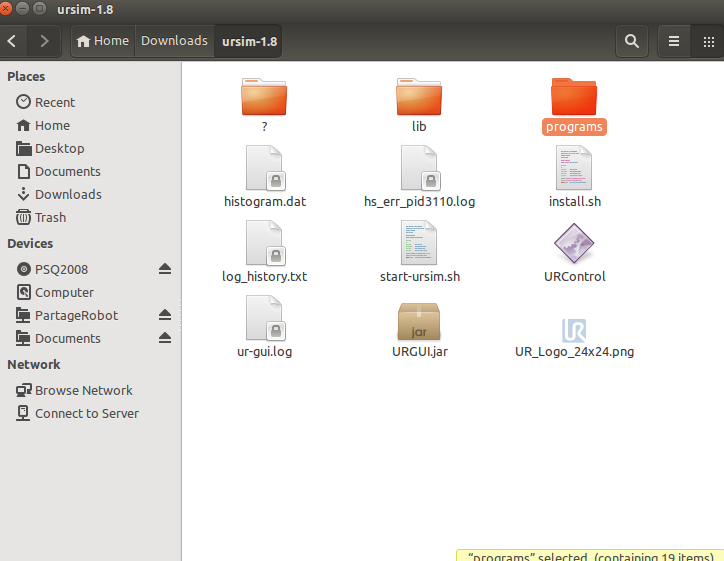
\includegraphics[trim=0cm 0cm 0cm 0cm, scale=0.5]{screenshots_tuto_ursim/programs.png}
  \end{tabular}
 \end{center}
\caption{Emplacement du dossier \textit{programs}}
 \label{fig:programs}
\end{figure}
Suivant le dépot du dossier \textit{programs} dans le répertoire d'URsim, il est possible d'ouvrir le programme portant le nom
\textit{matlabcontrolV3.urp} après avoir sélectionné \textit{Load Program} tel que vu dans la Figure \ref{fig:ui_start}.

Ensuite, il faut executer les étapes suivante:
\begin{itemize}
\item Modifier l'adresse IP dans la fonction \textit{socket\_open} du URscript pour qu'elle concorde avec l'adresse IP du controleur réseau de VMware. Cette infromation est disponible en ouvrant un invité de commande dans la session Windows et de tapper ipconfig. La Figure \ref{fig:windows_ip} représente la sortie de l'invité de commande qu'il faut remarquer lors de l'envoie de la commande ipconfig.
\item Sélectionner l'option \textit{Simulation} dans le bas de la fenêtre d'URsim.
\item Appuyer sur le bouton \textit{Play} présent de le bas, au centre, de la fenêtre d'URsim.
\end{itemize}
\begin{figure}
 \begin{center}
  \begin{tabular}{c}
    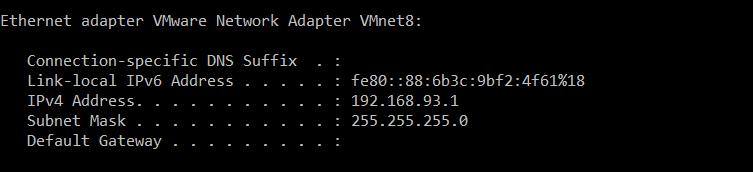
\includegraphics[trim=0cm 0cm 0cm 0cm, scale=0.5]{screenshots_tuto_ursim/windows_ip.png}
  \end{tabular}
 \end{center}
\caption{Exemple de l'adresse ip du contrôleur de VMware qu'il faut prendre en note (IPv4 address)}
 \label{fig:windows_ip}
\end{figure}
Ces étapes lancent l'URscript sur un robot virtuel et permet l'écoute et la réponse à des commandes envoyées par Matlab.


\subsubsection{Interface Matlab-URsim}

Une fois l'environnement virtuel d'URsim mis en place, l'environement matlab requis pour communiquer avec URsim doit être implémenté.
Un environnement de travail matlab situé dans le répertoire github mentionné plus dans la dernière section contient plusieurs fichiers nécessaires à la communiquation avec URsim.

Un survol rapide du URscript \textit{matlabcontrolV3.urp} permet d'observer qu'URsim attend l'arrivée de différents types de packets et détermine la commande à accomplir avec la valeur de la première donnée comprise dans une liste de longueur prédéterminée. Les fichiers Matlab permettant de faire le lien avec URsim font seulement traduire les arguments dans la forme qui rend possible la lecture par VRep.

Voici la liste des fonctions disponible dans le répertoire github fourni: 
\begin{itemize}
\item Robot\_Pose\_j $=$ readrobotpose\_j(Socket\_conn).	Lecture des position articulaires du robot.
\item Robot\_Pose $=$ readrobotpose(Socket\_conn).			Lecture de la position à l'effecteur du robot.
\item Robot\_Pose\_new $=$ moverobot(Socket\_conn,Goal\_Pose,Orientation).	Envoie de commande en position articulaires.
\item Robot\_speed $=$ readrobotspeed(Socket\_conn).		Lecture des vitesses cartésiennes du robot.
\item Robot\_speed\_j $=$ readrobotspeed\_j(Socket\_conn).	Lecture des vitesses articulaires du robot.
\item Robot\_speed\_j\_new $=$ speedrobot(Socket\_conn,theta\_dot). Envoie de commande en vitesse articulaires.
\item inv\_kin $=$ getinversekin(Socket\_conn,next\_pose).	Calcul de la cinématique inverse du UR5.
\end{itemize}



Ces fonctions permettent l'appel des fonctions d'URsim listées dans l'annexe A.
Une fois les packets lus par URsim, le URscript détermine quelle fonction appeler.
Suivant la méthodologie utilisée, il est facile d'ajouter des fonctions au URscript et d'adapter des fonctions Matlab à la nouvelle commande à envoyer.

\subsection{Logiciel de visualistion VRep}

Bien que le logiciel URsim permet de représenter le robot dans un environnement 3D de base, il ne permet pas la représentation d'objets composant l'environnement de travail du robot.
Pour se faire, le logiciel VRep est utilisé.
Ce dernier permet d'afficher une multitude d'objets localisés dans une librairie déjà prédéfinie.
Cette section couvre brièvement les étapes requise pour l'instalation et l'utilisatiuon de VRep avec matlab.
Il est à noter que VRep peut également servir de simulateur pour le UR5, cependant, il n'est pas aussi fidèle qu'URsim pour représenter les limitation en couple, courrant ou les arrêts d'urgence.

\subsubsection{Instalation de VRep}

L'instalation de VRep peut se faire rapidement en téléchargeant la version d'éducation sur le site web officiel \href{http://www.coppeliarobotics.com/downloads.html}{suivant}.

\subsubsection{Interface Matlab-VRep}

VRep est doté d'une API très versatile pouvant être utilisée dans plusieurs langages de programation tels que C/C++, Python, Matlab, Java, Octave et Lua.
Pour avoir accès aux fonction de l'API dans un projet Matlab, il faut aller chercher les fichiers suivants:
\begin{itemize}
\item remApi.m
\item remoteApiProto.m
\item remoteApi.dll
\end{itemize}

Ces fichiers sont situés dans les dossiers d'instalation de VRep.
Sur le système d'exploitation Windows, cet endroit est normalement: 
\newline
C:\textbackslash Program Files (x86)\textbackslash V-REP3\textbackslash V-REP\_PRO\_EDU\textbackslash programming\textbackslash remoteApiBindings\textbackslash matlab\textbackslash matlab
\newline
pour le fichier ".m" et:
\newline
C:\textbackslash Program Files (x86)\textbackslash V-REP3\textbackslash V-REP\_PRO\_EDU\textbackslash programming\textbackslash remoteApiBindings\textbackslash lib\textbackslash lib\textbackslash 64Bit
\newline
pour le fichier ".dll".
\newline

Suite à l'incorporation de ces fichiers dans l'environnement de travail, il est possible d'initialiser l'objet interagissant avec l'API dans matlab avec cette commande:
\newline

vrep=remApi('remoteApi');
\newline

Ensuite, il est possible d'envoyer des commandes à une instance de VRep.
Dans l'environnement du simulateur, l'interaction du script matlab avec VRep se résume à l'envoie des positions articulaires lues dans URsim.

\subsection{Exemple d'utilisation}

Les étapes suivantes réfèrent aux scripts matlab situés dans le dossier \textit{URsim-vrep-matlab} du dépot github mentionné plus haut.
L'utilisation de la solution présentée dans cette section peut être résumée par les étapes suivantes:

\begin{itemize}
\item Connection d'un joystick dans l'ordinateur (requis pour l'exemple).
\item Ouverture de la machine virtuelle et démarage d'URsim
\item Chargement du URscript dans URsim.
\item Ouverture de VRep sur la session windows.
\item Chargement de la scène \textit{scene\_ur5\_1.ttt} dans VRep.
\item Démarage du script matlab nommé \textit{Exemple\_controle\_ur5\_vrep.m}.
\item Appuyer sur le bouton "play" de URsim
\end{itemize}

Suite à l'exécution de ces étapes, le robot est contrôlable avec le joystick et devrait être visualisé dans VRep. La Figure \ref{fig:vrep_scene} représente l'interface VRep lorsque la scène est chargée.
\begin{figure}
 \begin{center}
  \begin{tabular}{c}
    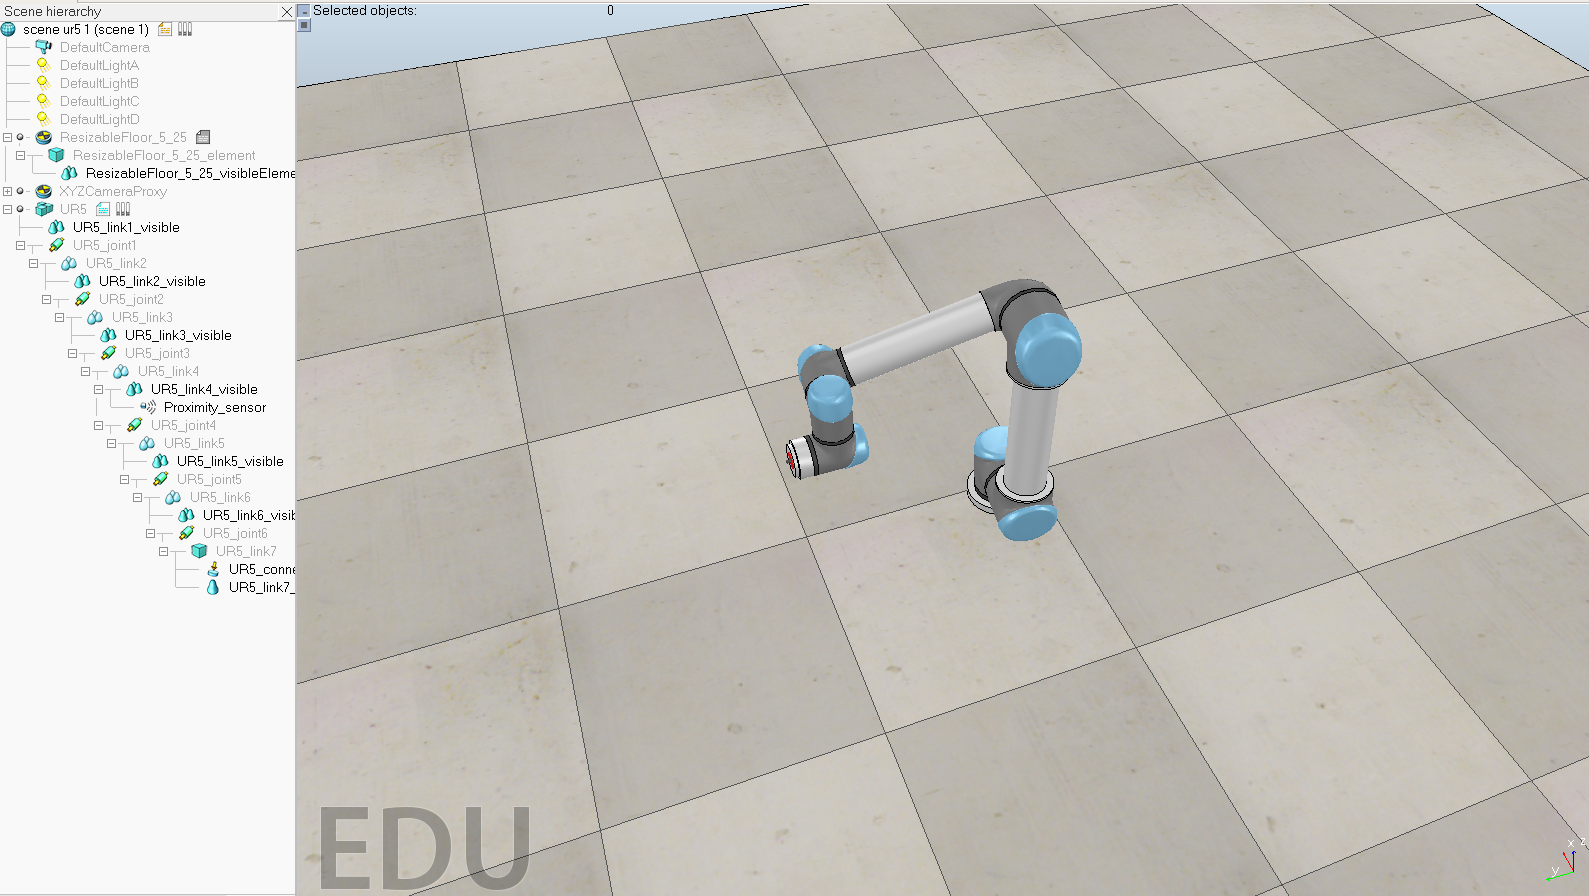
\includegraphics[trim=0cm 0cm 0cm 0cm, scale=0.25]{vrep_ur.png}
  \end{tabular}
 \end{center}
\caption{Interface du simulateur VRep avec la scène chargée.}
 \label{fig:vrep_scene}
\end{figure}
Pour plus de détails quant à l'utilisation des fonctions dans matlab, il est possible de lire le code exemple qui a été commenté pour faciliter la compréhension. De plus, l'annexe B est constituée d'un document listant la magoritée des commandes disponibles.

\subsection{Conclusion}

La solution de contrôle du bras UR5 avec matlab à été présentée.
L'instalation et l'utilisation de URsim dans une machine virtuelle à été abordée.
Cependant la nécessité d'utiliser une machine virtuelle ainsi qu'un logiciel de visualisation tel que VRep est quelque peu compliquée.


\newpage


\end{document}

















